\documentclass{article}
\usepackage{graphicx}
\usepackage{booktabs}
\usepackage{amsmath,amssymb}
\usepackage{hyperref}
\newcommand{\theHalgorithm}{\arabic{algorithm}}
\usepackage[accepted]{icml2025}
\usepackage{fontspec}
\setmainfont{Times New Roman}
\setsansfont{Arial}
\setmonofont[Scale=0.83]{Courier New}
\newfontfamily\cyrillicfonttt[Scale=0.83]{Courier New}
\usepackage{polyglossia}
\setdefaultlanguage{russian}
\setotherlanguage{english}
\setcitestyle{numbers,square,comma}
\hypersetup{pdftitle={Поиск объявлений услуг Авито},pdfauthor={},pdfsubject={Технический отчёт по конкурсу},colorlinks=true,urlcolor=blue,citecolor=blue,linkcolor=blue}
\makeatletter
\renewcommand{\Notice@String}{Технический отчёт по конкурсу. Использован макет ICML 2025. Документ не является публикацией ICML.}
\def\fnum@figure{Рисунок \thefigure}
\def\fnum@table{Таблица \thetable}
\makeatother
\renewenvironment{abstract}{\centerline{\large\bfseries Аннотация}\vspace{-0.12in}\begin{quote}}{\par\end{quote}\vskip 0.12in}
\icmltitlerunning{Поиск объявлений услуг Авито}
\newcommand{\ev}[1]{\href{https://github.com/revefffect/avito-contest/blob/main/evidence/INDEX.md\#E#1}{[E#1]}}
\newcommand{\file}[1]{\texttt{\small #1}}
\graphicspath{{figures/}}
\setlength{\emergencystretch}{1em}

\begin{document}
\raggedbottom
\twocolumn[
\icmltitle{Поиск объявлений услуг Авито:\\метод, результаты и проверка воспроизводимости}
\begin{center}
Технический отчёт по конкурсному решению\\
28 сентября 2026 года
\end{center}
\vskip 0.15in
]
\begingroup
\renewcommand\thefootnote{}
\footnotetext{Технический отчёт по конкурсу. Использован макет ICML 2025. Документ не является публикацией ICML.}
\endgroup

\begin{abstract}
Для каждого поискового запроса требуется вернуть не более 50 объявлений из заданного корпуса. Решение объединяет словный и символьный поиск, BM25, эмбеддинги multilingual-e5-small, географию и статистики обучающих взаимодействий. Две модели CatBoost отбирают итоговые объявления. На независимой локальной выборке из 1500 запросов выбранная смесь получила Recall@50, равный 0{,}941111. Полнота объединённого набора до отбора 50 составила 0{,}988667. Параметры зафиксированы до просмотра этой выборки. Мини-ноутбук применяет сохранённые модели и признаки, затем проверяет SHA256 сформированного CSV. Значение метрики на скрытом benchmark неизвестно. Источники результатов доступны в индексированном наборе доказательств \ev{014}\ev{015}\ev{016}.
\end{abstract}

\section{Задача и критерий качества}

В условии конкурса предоставлены обучающие пары запроса и выбранного объявления, неразмеченные запросы benchmark и корпус объявлений. Для каждого запроса нужен список из не более чем 50 исходных \file{item\_id}. Идентификаторы сохраняются строками, регистр и ведущие нули существенны \ev{001}.

Пусть $Q$ обозначает набор запросов, $R(q)$ содержит все известные релевантные объявления, а $T_{50}(q)$ содержит предсказанные 50. Целевая метрика равна
\begin{equation}
\operatorname{Recall@50}=\frac{1}{|Q|}\sum_{q\in Q}
\frac{|T_{50}(q)\cap R(q)|}{|R(q)|}.
\label{eq:recall}
\end{equation}
Среднее берётся по запросам. Запрос с несколькими положительными объявлениями не получает больший вес. Если нужное объявление не найдено генератором кандидатов, оно остаётся в знаменателе и снижает итоговый Recall \ev{015}.

\section{Данные и признаки}

Размеры исходных файлов приведены в таблице~\ref{tab:data}. В train наблюдаются 344825 различных объявлений. Первичный профиль даёт 73873 текста после приведения к нижнему регистру, замены ё и сведения пробелов. Полный нормализатор поиска дополнительно применяет NFKC и извлекает буквенно-числовые токены, получая 73706 текстов. Два числа относятся к разным правилам обработки \ev{032}. Наблюдаемая пара означает выбор пользователя, но отсутствие пары не доказывает нерелевантность объявления \ev{003}.

\begin{table}[t]
\caption{Исходные данные. Числа проверяются по Parquet и профилю данных.}
\label{tab:data}
\centering
\small
\begin{tabular}{lr}
\toprule
Файл & Число строк \\
\midrule
\file{train.parquet} & 497673 \\
\file{benchmark\_queries.parquet} & 2452 \\
\file{benchmark\_items.parquet} & 189212 \\
\bottomrule
\end{tabular}
\end{table}

Текст запроса, фильтры, заголовок, параметры и описание объявления нужны для тематического соответствия. Локация и координаты помогают отличать местные услуги от удалённых. Статистики похожих запросов дают распределение подкатегорий даже для новых объявлений. Цена, рейтинг, число отзывов и доступность связи дополняют текстовые оценки. Модель не получает идентификаторы или позицию объявления в корпусе \ev{027}.

По первичному профилю в benchmark 37{,}36\% текстов запросов уже встречались в train, а полный контекст встречался в 4{,}40\% случаев. Контекст включает текст, локацию, доставку, фильтры и категорию. В train встречались только 9{,}59\% объявлений корпуса. Последнее число относится ко всему корпусу. Доля знакомых объявлений среди скрытых правильных ответов неизвестна \ev{003}.

Буквальное совпадение категории исключено из итоговых моделей. Категория поиска 0 встречается лишь в 34 строках train, но в 222 запросах benchmark. В корпусе нет объявлений категории 0. Все 34 известные положительные пары такого поиска относятся к категории 114. Смысл кода 0 не подменяется догадкой, вместо этого модель не получает нестабильный признак равенства категорий \ev{005}.

\section{Как устроен поиск}

\subsection{Источники кандидатов}

Нормализация переводит текст в нижний регистр, заменяет букву ё на е и сохраняет числа и латиницу. Русские слова обрабатываются SnowballStemmer из NLTK~\citep{nltk}. Словный TF-IDF использует слова и биграммы из заголовка и параметров. Символьный TF-IDF по фрагментам длиной от 3 до 5 символов дополняет поиск при близких написаниях~\citep{sklearn}.

BM25 учитывает заголовок, параметры и первые 3000 символов описания. Заголовок повторяется трижды, параметры дважды. Используются положительный IDF, $k_1=1{,}2$ и $b=0{,}65$. Дополнительный признак покрытия показывает долю разных токенов запроса, найденных в индексируемом тексте. Повторы одного слова не увеличивают эту долю \ev{027}.

Модель multilingual-e5-small применяется локально без дообучения~\citep{e5}. Запрос кодируется с фильтрами и отдельно без них. Объявление кодируется как заголовок, параметры и начало описания. Префиксы \file{query:} и \file{passage:}, усреднение токенов с учётом маски и нормализация векторов следуют карточке модели. Порядок полей и ограничения входа выбраны в этом решении.

Векторы имеют размерность 384. Для объявления используются не более 256 токенов, для запроса 128. Сохранённые векторы рассчитаны в float32 на Apple MPS пакетами по 64 текста. Ревизия модели и хеши весов зафиксированы. Проверка обнаружила конечные значения во всех массивах и максимальную ошибку единичной нормы $1{,}79\cdot10^{-7}$ \ev{018}.

Кандидаты отбираются глобально и с географической поправкой. В объединение входят BM25, оба TF-IDF, поиск по запросу с фильтрами, обе версии E5 и выборы похожих обучающих запросов. После удаления повторов на dev остаётся в среднем 1121{,}07 кандидата. В benchmark среднее равно 1062{,}25 \ev{011}\ev{034}.

\subsection{География и история}

Совпадение локаций наблюдается в 83{,}10\% положительных обучающих пар. У 17{,}41\% запросов benchmark нет объявлений с тем же идентификатором локации. Поэтому расстояние используется как мягкий признак \ev{004}.

Центр локации оценивается по медиане координат объявлений. Для локации запроса без собственного центра используются обучающие переходы. Признаки включают расстояние, вероятность перехода и её отношение к общей частоте локации. Ширина поиска зависит от разброса наблюдаемых переходов. Правила для отдельных идентификаторов не задаются.

История похожих запросов даёт кандидатов, вероятности подкатегорий и поддержку фильтров. Первая итоговая модель также использует популярность объявления, счётчики пар с текстом и контекстом, оценку поведенческого источника и его позиции. Вторая исключает шесть прямых признаков истории объявления. Остальные агрегаты и общий набор кандидатов у моделей совпадают \ev{014}.

\subsection{Отбор 50 объявлений}

Обучается \file{CatBoostClassifier} с функцией потерь Logloss~\citep{catboost}. Положительная пара получает метку 1, остальные кандидаты 0. Неполная разметка означает, что некоторые нулевые метки могут соответствовать подходящим объявлениям.

Обе модели имеют глубину 6 и скорость обучения 0{,}07. Модель с прямой историей содержит 700 деревьев, другая 1000. Число деревьев выбрано по Recall@50 на dev. Случайное зерно равно 42 \ev{014}.

Перед смешиванием оценки стандартизуются внутри каждого запроса по всему набору кандидатов $C(q)$:
\begin{align}
\mu_m(q)&=\frac{1}{|C(q)|}\sum_{d\in C(q)}s_m(q,d),\\
\sigma_m^2(q)&=\frac{1}{|C(q)|}\sum_{d\in C(q)}(s_m(q,d)-\mu_m(q))^2,\\
z_m(q,d)&=\frac{s_m(q,d)-\mu_m(q)}{\sigma_m(q)},\\
s(q,d)&=0{,}5z_1(q,d)+0{,}5z_2(q,d).
\end{align}
При нулевом отклонении соответствующая оценка $z_m$ равна нулю. При равных итоговых оценках используется исходная позиция объявления. Такой порядок фиксирует результат повторного запуска \ev{021}\ev{027}.

\section{Проверка до отправки}

\subsection{Разделение и защита от утечки}

Из train выбраны 6000 контекстов с 6432 положительными парами. Первые 3000 запросов используются для обучения отбора, следующие 1500 для выбора настроек и последние 1500 для независимой проверки, называемой audit. Зерно разделения равно 20260928 \ev{006}.

Проверяемые пары удалены из истории до расчёта признаков. Для новых текстов скрыты все обучающие строки с этими текстами. Дополнительно удалена история случайно выбранных 90{,}4\% целевых объявлений. После совместного применения ограничений 96{,}56\% положительных проверочных пар относятся к объявлениям без оставшейся истории. Такая доля служит допущением стресс-теста и не считается известным свойством скрытого benchmark \ev{006}.

Поиск проверяется на полном корпусе benchmark с добавлением 5913 отложенных объявлений из train. Всего доступны 195125 документов. Маленькая случайная выборка негативов не используется. Тексты отложенных объявлений доступны индексам, а факты их выбора скрыты от поведенческих статистик. Повторная сборка разделения дала побайтно одинаковые четыре Parquet-файла \ev{007}.

Независимая сверка обнаружила 22 целевых идентификатора объявлений, общих для fit с dev и audit. Поэтому части раздельны по запросам, но не полностью по объявлениям. После исключения 22 затронутых запросов остаются 1478 запросов с 1573 положительными парами. На них Recall@50 равен 0{,}941249, а оценка с поправкой на фильтры 0{,}942929. Чувствительность рассчитана без переобучения и изменения выбранной модели. Протокол приведён в \file{report/independent\_audit.json} \ev{032}.

\subsection{Поправка на различие запросов}

В benchmark доля запросов без фильтров равна $p=0{,}6305057$. В локальной проверке она ниже. Дополнительно рассчитывается
\begin{equation}
R_{\mathrm{adj}}=pR_{\mathrm{empty}}+(1-p)R_{\mathrm{filtered}}.
\end{equation}
Веса определены по открытым признакам benchmark. Поправка учитывает только наличие фильтров и не устраняет другие различия распределений \ev{013}.

\section{Результаты и ошибки}

\begin{figure}[t]
\centering
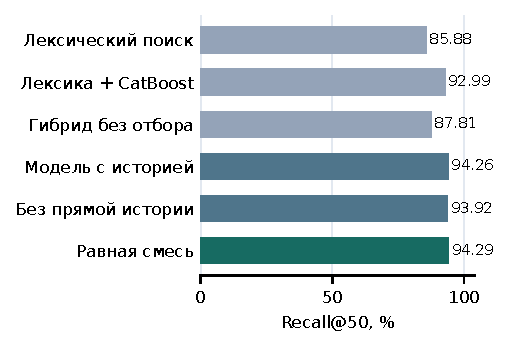
\includegraphics[width=\columnwidth]{dev.pdf}
\caption{Развитие решения на dev. Этапы используют одну разметку, но расширенный гибридный поиск имеет другой набор кандидатов. Прибавку между этапами нельзя целиком приписать одному новому компоненту \ev{008}\ev{009}\ev{011}\ev{013}.}
\label{fig:dev}
\end{figure}

Исходный лексический поиск с географией получил Recall@50 0{,}858833. На том же сохранённом наборе кандидатов CatBoost повысил результат до 0{,}929889. Следовательно, значительная часть исходных ошибок связана с отбором 50 из уже найденных объявлений \ev{008}\ev{009}.

В исходном разборе 177 положительных пар находились среди кандидатов ниже 50-го места, а 53 отсутствовали в объединении. Из 53 пропусков у 26 не было словного пересечения с запросом. Для этих случаев добавлены два представления E5 и расширены географические словные источники. Полнота объединения на dev выросла с 0{,}966778 до 0{,}989333. Отдельного опыта, изолирующего весь вклад E5, не проводилось \ev{008}\ev{011}\ev{023}.

Фильтры и вероятности подкатегорий помогают отбирать тематически близкие услуги. Покрытие полного текста добавлено потому, что нужная услуга может быть описана в теле объявления при общем заголовке. Глобальное ослабление географического штрафа ухудшало исходный Recall до 0{,}824389, поэтому сохранён мягкий локальный поиск с признаками ширины и переходов \ev{023}.

На dev модель с прямой историей получила 0{,}942611, модель без неё 0{,}939167, а равная смесь 0{,}942944. Преимущество смеси над первой моделью составило лишь 0{,}000333. Парный bootstrap с 2000 повторов дал 95-процентный интервал разницы от $-0{,}004333$ до $0{,}005000$. Превосходство статистически не подтверждено \ev{013}.

\begin{table}[t]
\caption{Независимая проверка после обучения на 4500 запросах. Настройки после просмотра audit не менялись \ev{014}\ev{015}.}
\label{tab:audit}
\centering
\small
\begin{tabular}{lrr}
\toprule
Модель & Recall@50 & $R_{\mathrm{adj}}$ \\
\midrule
С прямой историей & 0{,}939778 & 0{,}941560 \\
Без прямой истории & 0{,}946417 & 0{,}948674 \\
Основная смесь & 0{,}941111 & 0{,}943178 \\
\bottomrule
\end{tabular}
\end{table}

\begin{figure}[t]
\centering
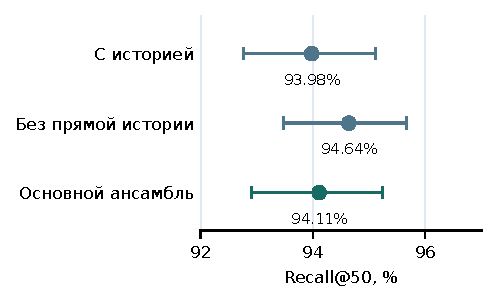
\includegraphics[width=\columnwidth]{audit.pdf}
\caption{Recall@50 на audit и 95-процентные интервалы percentile bootstrap по запросам, 5000 повторов. Интервалы описывают разброс локальной оценки и не покрывают неизвестный сдвиг скрытого теста \ev{016}.}
\label{fig:audit}
\end{figure}

Перед независимой проверкой выбранные модели переобучены на fit и dev, всего на 4500 запросах. Таблица~\ref{tab:audit} показывает результаты audit. Вариант без прямой истории оказался выше, хотя на dev был ниже. Основной ответ сохраняет заранее выбранную смесь. Для него 95-процентный bootstrap-интервал Recall@50 составляет от 0{,}9291 до 0{,}9524 \ev{014}\ev{015}\ev{016}.

\section{Воспроизведение и состав материалов}

Мини-версия находится в папке \file{mini}. В ноутбуке пять исполняемых ячеек: проверка файлов, загрузка кандидатов, применение моделей, отбор 50 и сохранение CSV. Для запуска нужны две модели CatBoost, списки признаков, числовая таблица кандидатов, две таблицы идентификаторов и конфигурация. Готовый CSV не используется для расчёта.

Код подготовки признаков и обучения сохранён отдельно в \file{reference\_solution}. Для полного пересчёта нужны исходный архив конкурса и закреплённые веса E5. Применение готовых моделей в мини-версии работает без внешних API после установки зависимостей. Полная пересборка эмбеддингов на CPU вместо MPS может дать численные отличия, поэтому её побайтовая переносимость между устройствами не заявляется \ev{018}\ev{020}.

Проверка исходного переносимого архива подтвердила хеши 74 файлов и повторно получила три CSV. Каждый содержит 2452 запроса по 50 объявлений. Все хеши ответов совпали с конфигурациями \ev{020}. Новый мини-ноутбук также выполнен в отдельной папке с чистым ядром Jupyter и без готового ответа. Все пять исполняемых ячеек завершились за 5{,}949 секунды, а SHA256 совпал с основным ответом. Протокол хранится в \file{report/notebook\_verification.json} \ev{033}.

Индекс \file{evidence/INDEX.md} связывает документы с исходниками измерений. В \file{evidence/claims.csv} каждому утверждению сопоставляются источник и поле данных. Набор \file{data\_dump} включает отчёты, результаты по отдельным запросам, конфигурации и журналы экспериментов. Для больших исходных файлов сохраняются путь, размер и SHA256. Повторная проверка доступна без переписывания методики по тексту статьи.

\section{Ограничения}

Выводы относятся к одной схеме разделения. Доля новых целевых объявлений в ней задана искусственно. Некоторые нулевые метки могут быть пропущенными положительными примерами. Длинные описания обрезаются, а короткие запросы иногда не позволяют восстановить причину выбора пользователя. Подбор числа деревьев и вариантов смеси по dev делает его результат оптимистичным, поэтому итоговая оценка приводится отдельно по audit.

Уровень уверенности в точности воспроизведения высокий при совпадающих артефактах и версиях библиотек. Уверенность в переносе локальной метрики на скрытый benchmark средняя. Платформа пока не предоставила оценку ответа. Запасной вариант без прямой истории сохранён для отдельного сравнения, его преимущество на скрытом тесте не предполагается.

\begin{thebibliography}{9}
\bibitem{e5} Intfloat. Multilingual E5 small, model card. Закреплённая ревизия 614241f622f53c4eeff9890bdc4f31cfecc418b3. \url{https://huggingface.co/intfloat/multilingual-e5-small}.
\bibitem{catboost} CatBoost. CatBoostClassifier и применение моделей. \url{https://catboost.ai/docs/en/concepts/python-quickstart}.
\bibitem{sklearn} Scikit-learn. Text feature extraction, TF-IDF. \url{https://scikit-learn.org/stable/modules/feature_extraction.html}.
\bibitem{nltk} NLTK. Snowball stemmers. \url{https://www.nltk.org/api/nltk.stem.snowball.html}.
\end{thebibliography}

\end{document}
